
\subsection{Final State Interactions}

In order to accurately determine the nucleonic components of the deuteron's wave function, it is vital that final state interactions (FSI) are understood. As demonstrated below, FSI can introduce a significant component to $A_{zz}$, particularly in the large $x>1.2$ region. Including these effects is necessary for further constraining our theoretical understanding of the deuteron through $A_{zz}$.

The effects of FSI on $A_{zz}$ have recently been modeled by W. Cosyn in the deep-inelastic region~\cite{Cosyn:2014sqa} and in the quasi-elastic region discussed in this proposal~\cite{cosyn-convo}, which is an on-going area of research. Results are shown in Fig.~\ref{fig:fsi-kin1}-\ref{fig:fsi-kin2}. The calculations use the virtual nucleon (VN) approximation to compute inclusive observables in electron-induced scattering off the deuteron including the 
effect of final-state interactions. Amplitudes and observables are computed in an unfactorized manner.   

Current calculations include on-shell and off-shell contributions to the FSI amplitudes, but the off-shell contribution is calculated by neglecting any  possible singularities of the EM current in the complex plane.  Calculations 
including these are forthcoming.  The inclusive observables are computed using 
the optical theorem in a manner analogous to Ref.~\cite{Cosyn:2013uoa}.  The 
rescattering of the struck nucleon with the spectator is modeled using an 
eikonal amplitude.  For the calculations included in this proposal, the off-shell 
contribution to the FSI amplitude has not been suppressed in any manner, such that the maximum possible effect of FSI are estimated.

\begin{figure}[htb]
\begin{center}
  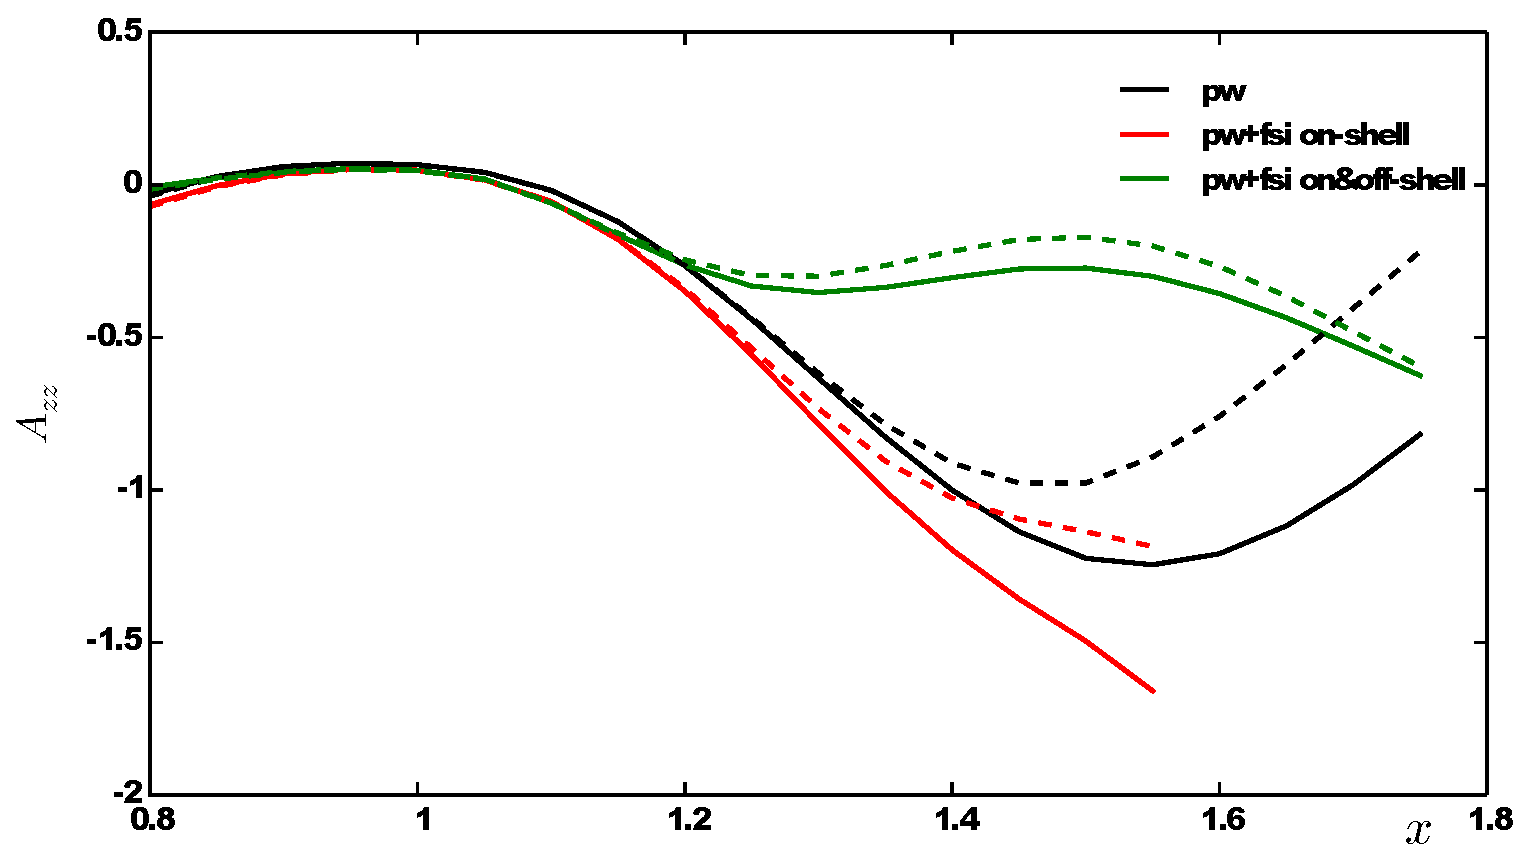
\includegraphics[width=0.5\textwidth]{figs/kin1_cdbonn_av18.eps}
\caption{$A_{zz}$ calculation for $E_0=8.8\mathrm{~GeV}^2$ and $Q^2=1.5\mathrm{~(GeV/}c)^2$ including contributions from final state interactions.  
Solid curves were calculated using the CDBonn deuteron wave function, dashed curves using the AV18 
deuteron wave function.}
\label{fig:fsi-kin1}       % Give a unique label
\end{center}
\end{figure}

\begin{figure}[htb]
\begin{center}
  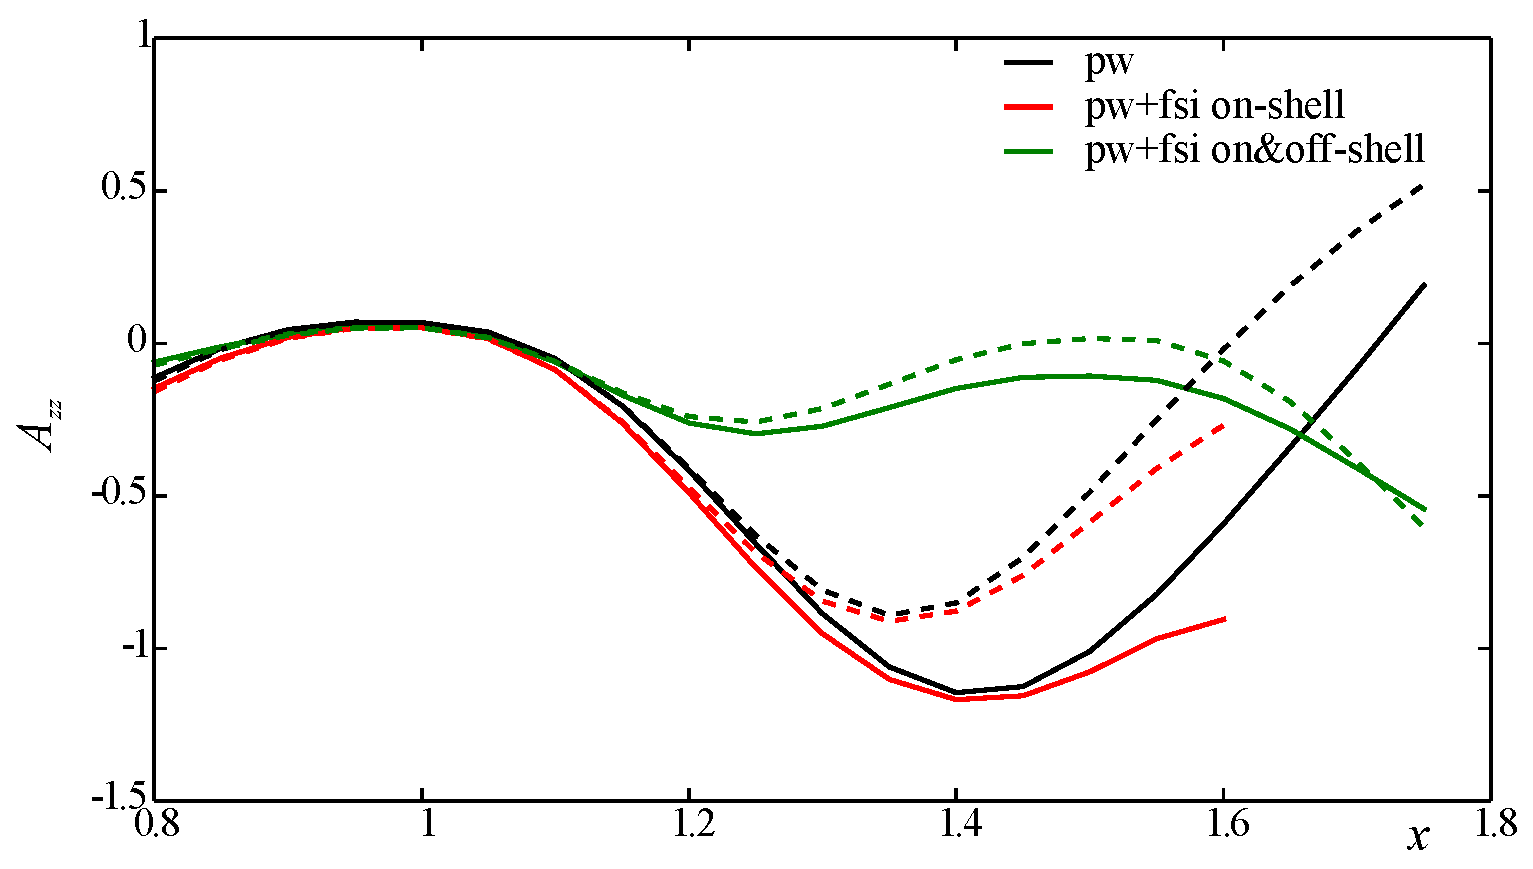
\includegraphics[width=0.5\textwidth]{figs/kin2_cdbonn_av18.eps}
\caption{Same as Fig.~\ref{fig:fsi-kin1}, but for $E_0=8.8\mathrm{~GeV}^2$ and $Q^2=2.9\mathrm{~(GeV/}c)^2$.}
\label{fig:fsi-kin2}       % Give a unique label
\end{center}
\end{figure}

%Note: strange bumps in the red curves (plane-wave+on-shell fsi) is due to contributions almost cancelling each other in combination with numerical errors.  Which means the numerical noise gets enhanced bigtime.  I suggest dropping these for now, since the off-shell contribution dominates anyway.

\iffalse
Most theory calculations calculate Azz with a deuteron polarized along the  virtual photon momentum direction as this limits the number of response  functions included in the cross section.  For a deuteron polarized along the  electron beam direction, an extra rotation of the deuteron density matrix needs  to be accounted for and extra response functions contribute~\cite{Cosyn:2014sqa}.  The next figures show how $A_{zz}$ changes  when accounting for this.

\begin{figure}[htb]
\begin{center}
  \includegraphics[width=0.5\textwidth]{figs/beampol_av18_kin1.eps}
\caption{$A_{zz}$ calculation for kinematic S1 including FSI contributions 
using the AV18 wave function.  
Full curves use have a deuteron polarized along the photon direction, dashed 
ones along the electron beam.}
\label{fig:beampol1}       % Give a unique label
\end{center}
\end{figure}

\begin{figure}[htb]
\begin{center}
  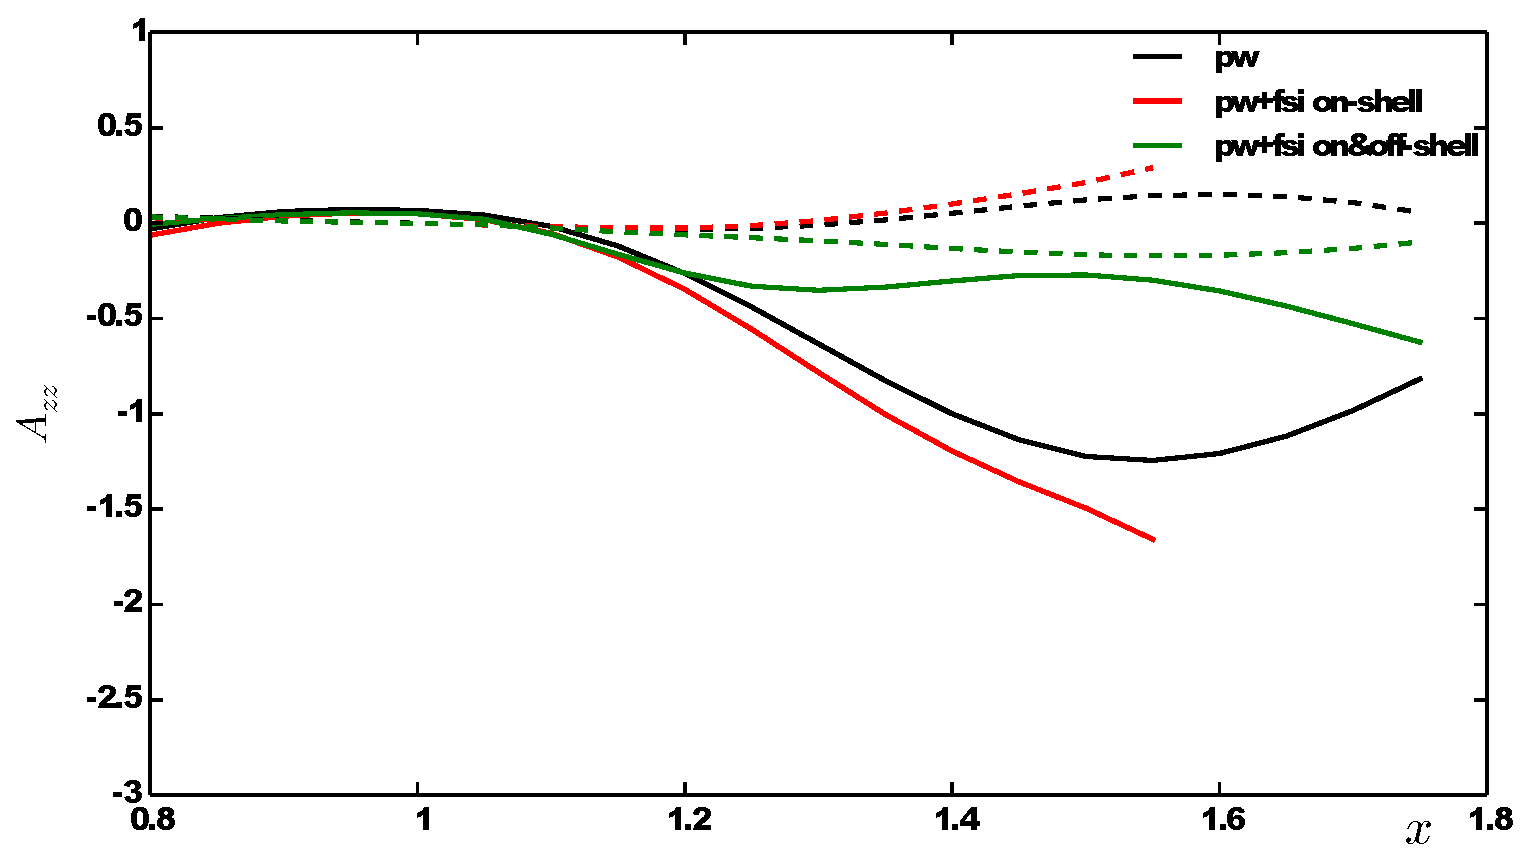
\includegraphics[width=0.5\textwidth]{figs/beampol_cdbonn_kin1.eps}
\caption{Same as Fig.~\ref{fig:beampol1}, but for cdbonn wave function.}
\label{fig:beampol2}       % Give a unique label
\end{center}
\end{figure}

\begin{figure}[htb]
\begin{center}
  \includegraphics[width=0.5\textwidth]{figs/beampol_av18_kin1.eps}
\caption{Same as Fig.~\ref{fig:beampol1}, but H1 kinematics and AV18 wave 
function.}
\label{fig:beampol3}       % Give a unique label
\end{center}
\end{figure}

\begin{figure}[htb]
\begin{center}
  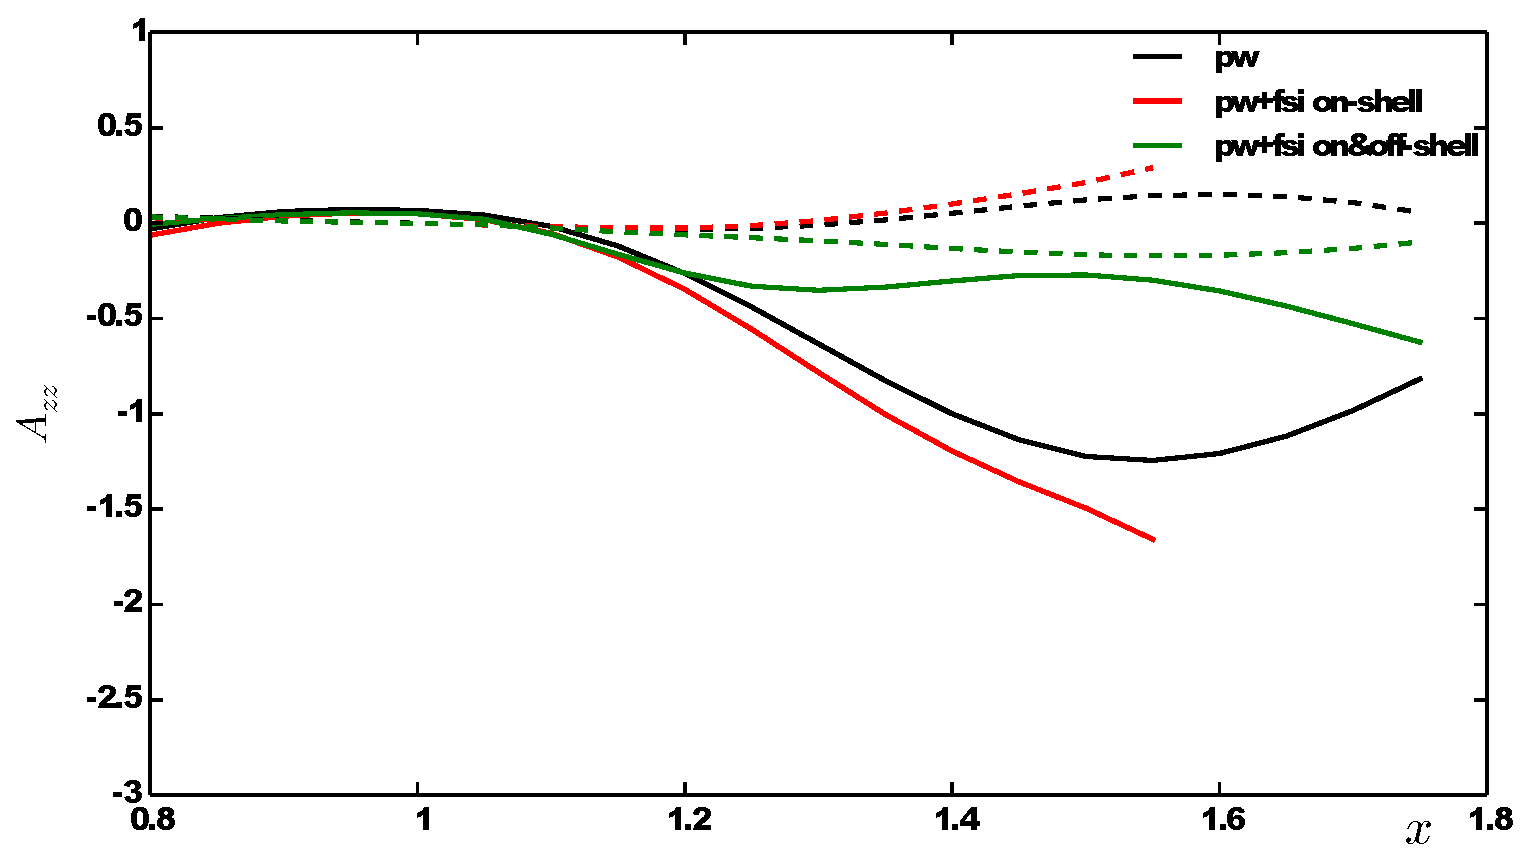
\includegraphics[width=0.5\textwidth]{figs/beampol_cdbonn_kin1.eps}
\caption{Same as Fig.~\ref{fig:beampol1}, but H1 kinematics and cdbonn wave 
function.}
\label{fig:beampol4}       % Give a unique label
\end{center}
\end{figure}
\fi

